\documentclass[t,xcolor={table},fleqn]{beamer}

\mode<presentation>
{
  \usetheme[deutsch,titlepage0]{KIT}
% \usetheme[usefoot]{KIT}
% \usetheme{KIT}

%%  \usefonttheme{structurebold}

  \setbeamercovered{transparent}

  %\setbeamertemplate{enumerate items}[circle]
  \setbeamertemplate{enumerate items}[ball]

}
\usepackage{babel}

\newlength{\Ku}
\makeatletter
\setlength{\Ku}{1.43375pt}
\makeatother

\usepackage[utf8]{inputenc}
\usepackage[TS1,T1]{fontenc}
\usepackage{array}
\usepackage{multicol}

\usepackage[                 % !! what about the ``biblatex.cfg''?
    backend=bibtex8,      % (bibtex), bibtex8, biber
    style=authoryear,		 %numeric-comp,
	maxcitenames=2,      % sets the maximum numbers of authors before abbreviated to et al in text
	maxbibnames=25,       % sets the maximum numbers of authors before abbreviated to et al in bibliography
    bibencoding=inputenc,   % (ascii), inputenc, <encoding>
    uniquename=init,   % true, (false), init
    doi=false,
    url=false,
	isbn = false,
    giveninits = true % render first/middle names as initals
]{biblatex}
\renewcommand*{\bibfont}{\footnotesize}
\setbeamertemplate{bibliography item}{}

\bibliography{../doc/tex/library,../doc/tex/urls}

%myStuff
\usepackage{amsthm}
\usepackage{amsmath,amssymb,bbm}
\usepackage{KITKaesten}
\usepackage{enhKITbeamer}

\usepackage{helvet}

%\usepackage[table]{xcolor}
\usepackage{url}
\usepackage{eso-pic}
\usepackage{caption}
\usepackage{subcaption}
\usepackage{makecell}
\usepackage{tabularx}
\usepackage{float}
\usepackage{pifont}

\definecolor{darkgreen}{HTML}{00B000}
\definecolor{darkred}{HTML}{D00000}
\newcommand{\cmark}{\color{darkgreen}\ding{51}}%
\newcommand{\xmark}{\color{darkred}\ding{55}}%

\definecolor{kit-green100}{rgb}{0,.59,.51}
\definecolor{kit-green70}{rgb}{.3,.71,.65}
\definecolor{kit-green50}{rgb}{.50,.79,.75}
\definecolor{kit-green30}{rgb}{.69,.87,.85}
\definecolor{kit-green15}{rgb}{.85,.93,.93}

\definecolor{kit-blue100}{rgb}{.27,.39,.67}
\definecolor{kit-blue70}{rgb}{.49,.57,.76}
\definecolor{kit-blue50}{rgb}{.64,.69,.83}
\definecolor{kit-blue30}{rgb}{.78,.82,.9}
\definecolor{kit-blue15}{rgb}{.89,.91,.95}

\definecolor{kit-yellow100}{cmyk}{0,.05,1,0}
\definecolor{kit-yellow70}{cmyk}{0,.035,.7,0}
\definecolor{kit-yellow50}{cmyk}{0,.025,.5,0}
\definecolor{kit-yellow30}{cmyk}{0,.015,.3,0}
\definecolor{kit-yellow15}{cmyk}{0,.0075,.15,0}

\definecolor{kit-orange100}{cmyk}{0,.45,1,0}
\definecolor{kit-orange70}{cmyk}{0,.315,.7,0}
\definecolor{kit-orange50}{cmyk}{0,.225,.5,0}
\definecolor{kit-orange30}{cmyk}{0,.135,.3,0}
\definecolor{kit-orange15}{cmyk}{0,.0675,.15,0}

\definecolor{kit-red100}{cmyk}{.25,1,1,0}
\definecolor{kit-red70}{cmyk}{.175,.7,.7,0}
\definecolor{kit-red50}{cmyk}{.125,.5,.5,0}
\definecolor{kit-red30}{cmyk}{.075,.3,.3,0}
\definecolor{kit-red15}{cmyk}{.0375,.15,.15,0}

\usepackage{tikz}
\usetikzlibrary{shapes.geometric,arrows,positioning}

\tikzstyle{circle1} = [circle,draw=kit-green15,fill=kit-green15,inner sep=0pt,minimum size=.8cm]
\tikzstyle{circle2} = [circle,draw=kit-green30,fill=kit-green30,inner sep=0pt,minimum size=.8cm]
\tikzstyle{circle3} = [circle,draw=kit-green50,fill=kit-green50,inner sep=0pt,minimum size=.8cm]
\tikzstyle{circle4} = [circle,draw=kit-green70,fill=kit-green70,inner sep=0pt,minimum size=.8cm]
\tikzstyle{circle5} = [circle,draw=kit-green100,fill=kit-green100,inner sep=0pt,minimum size=.8cm]

%\tikzset{
%  invisible/.style={opacity=.4},
%  visible on/.style={alt={#1{}{invisible}}},
%  alt/.code args={<#1>#2#3}{%
%    \alt<#1>{\pgfkeysalso{#2}}{\pgfkeysalso{#3}} % \pgfkeysalso doesn't change the path
%  },
%}

\tikzstyle{neuron} = [circle,draw=black,fill=none,inner sep=0pt,minimum size=4mm]
\tikzstyle{arrow} = [thick,->,>=stealth]

\tikzset{%
  every neuron/.style={
    circle,
    draw,
    minimum size=.25cm
  },
  neuron missing/.style={
    draw=none, 
    scale=1,
    text height=0.1cm,
    execute at begin node=\color{black}$\vdots$
  },
}

\newcommand{\tcite}{\Textcite}
\newcommand{\acrs}{\acrshort}

\title{Evaluating the benefit of grid-based weather information in energy forecasting}
\subtitle{Marcel Herm}
\author{Marcel Herm}
\institute{INSTITUT FÜR AUTOMATION UND ANGEWANDTE INFORMATIK}
\TitleImage[width=\titleimagewd]{images/bulb}
\newlength{\tmplen}
\newcommand{\verysmall}{\fontsize{6pt}{8.6pt}\selectfont}

\begin{document}

\begin{frame}
  \maketitle
\end{frame}

\makeatletter
\makeatother

%\noKITFrame
\removeKITFrame


\begin{frame}<1>[label=toc]{Overview}
\vspace{1cm}
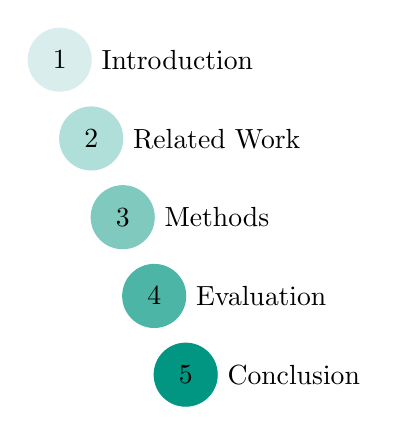
\begin{tikzpicture}[node distance=1cm]
  \node (fst) [circle1,label=0:Introduction] {1};
  \pause
  \node (snd) [circle2,below of=fst,xshift=.4cm,label=0:Related Work] {2};
  \pause
  \node (trd) [circle3,below of=snd,xshift=.4cm,label=0:Methods] {3};
  \pause
  \node (fth) [circle4,below of=trd,xshift=.4cm,label=0:Evaluation] {4};
  \pause
  \node (sth) [circle5,below of=fth,xshift=.4cm,label=0:Conclusion] {5};
\end{tikzpicture}

\end{frame}


\begin{frame}{Introduction}

\begin{figure}[h!]%
	\centering
	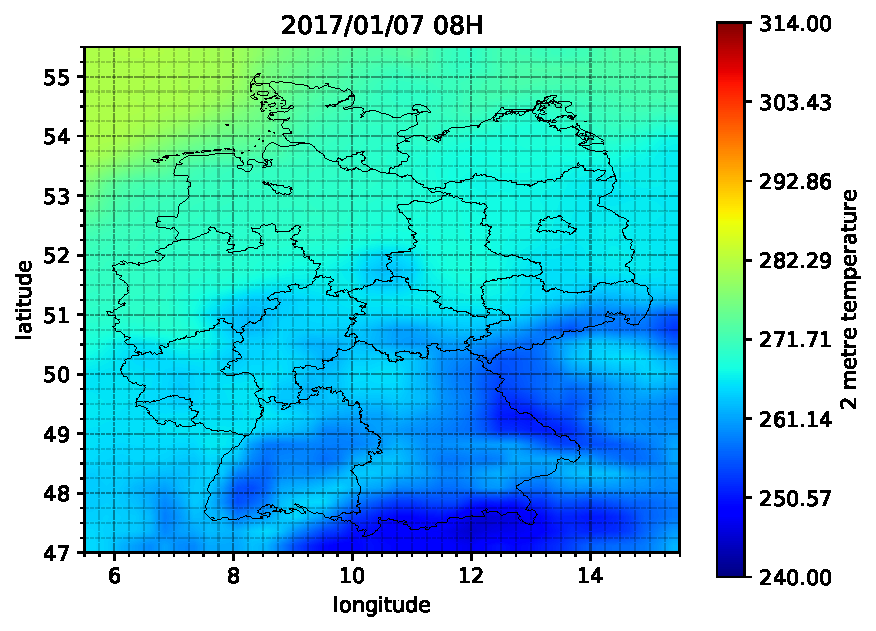
\includegraphics[height=.9\textheight]{../doc/plots/t2m/maxvar/0_map}%
\end{figure}

\end{frame}


\againframe<2>{toc}


\begin{frame}{Related Works}

%\vspace{20pt}
\begin{table}[!ht]%
\rowcolors{2}{white}{gray!25}
\centering
\scriptsize
\begin{tabularx}{\linewidth}{p{22mm}XXXX}
\textbf{paper} & \textbf{type of\newline weather data} & \textbf{forecast time\newline series} & \textbf{methods} & \textbf{forecast\newline horizon}\\\Xhline{2\arrayrulewidth}
\tcite{Ludwig2015} & station-based & energy prices & ARMA,ARMAX,\newline LASSO,RF & 24h\\
\tcite{Salcedo-Sanz2018} & grid-based & solar radiation & ELM,CRO,MARS,\newline MLR,SVR,GGA & 24h\\
\tcite{Diagne2013} & grid-based & solar radiation & ARMA,ARIMA,\newline CARDS,NN,WNN & 5 min-6h\\\Xhline{2\arrayrulewidth}
\tcite{Aguiar2016} & mixed & solar radiation & NN & 1-6h\\
\tcite{Bofinger2006} & mixed & solar power & MOS,IDW & 24-120h\\
\tcite{Haben2018} & station-based & low voltage\newline electricity load & KDE,SSLR,ARWD,\newline ARWDY,HWT & up to 4 days\\
\tcite{Alessandrini2015} & station-based & wind power & ANEN & 0-132h\\\Xhline{2\arrayrulewidth}
\tcite{Sperati2016} & grid-based & solar power & PDF,NN,VD,\newline EMOS,PE & 0-72h\\
\tcite{DeFelice2015} & grid-based & electricity\newline demand & LR,SVM & 1-2 months\\
\tcite{Davo2016} & grid-based & wind power,\newline solar radiation & PCA,ANEN,NN & 0-72h\\\Xhline{2\arrayrulewidth}
\textbf{This thesis} & grid-based & electricity load & ARMA,ARMAX & 1h\\
%\tcite{Aertsen2012} & mixed & \gls{ok},\gls{ck},\gls{rk} & long term & TODO\\ %  maybe not relevant du to only considering station-based measures and thus using interpolation methods (kriging)
%\tcite{Kaminska-Chuchmala2014} & distributed &  & & & \\
%\tcite{Fairley2017} & grid?! & methods?! & \gls{ecmwf} & none?! & TODO\\ % no forecast
%\tcite{Voivontas1998} & grid?! & & \gls{sdhws} & none?! & TODO\\
\end{tabularx}
\label{tab:relwork}
\end{table}

\end{frame}


\againframe<3>{toc}


\begin{frame}{Methodology}

\textbf{ARMA}
\begin{equation}
y_t = c+\sum_{i=1}^{p}\phi_iy_{t-i}+\sum_{j=1}^{q}\rho_j\epsilon_{t-j}+\epsilon_t
\end{equation}

\textbf{ARMAX}
\begin{equation}
y_t = c+\sum_{i=1}^{p}\phi_iy_{t-i}+\sum_{j=1}^{q}\rho_j\epsilon_{t-j}+\sum_{k=1}^{n}\eta_kx_k+\epsilon_t
\end{equation}

\textbf{Mean Absolute Percentage Error}
\begin{equation}
MAPE = \frac{1}{k}\times 100 \sum_{i=1}^{k} \left|\frac{y_i-\hat{y}_i}{y_i}\right|~.
\end{equation}

\end{frame}


\againframe<4>{toc}


\begin{frame}{Evaluation I}

Data filtered using shapefile from Eurostat\footnote{\url{https://ec.europa.eu/eurostat/de/web/gisco/geodata/reference-data/administrative-units-statistical-units/nuts}}.

\begin{figure}[h!]%
	\centering
	\begin{subfigure}{.5\textwidth}
		\centering
		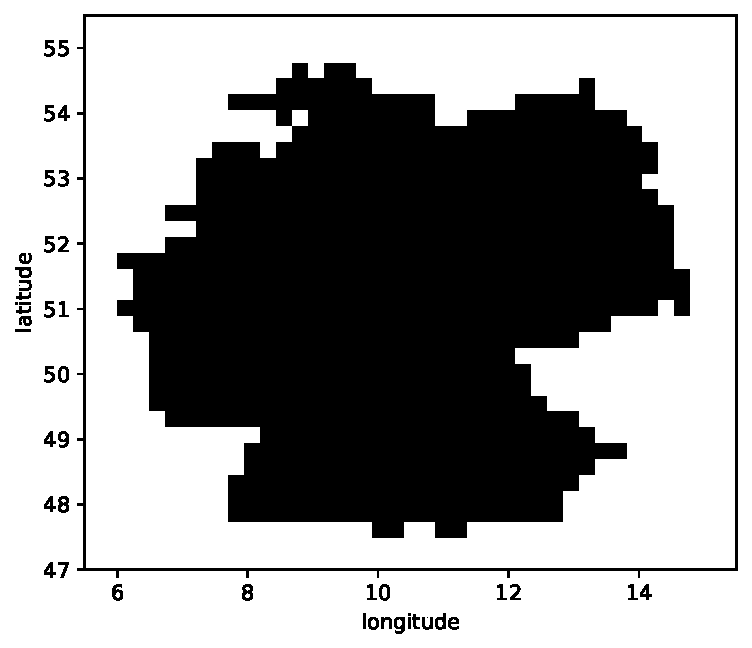
\includegraphics[width=.85\textwidth]{../doc/plots/isinDE}%
		\label{fig:isinDE}%
	\end{subfigure}%
	\begin{subfigure}{.5\textwidth}
		\centering
		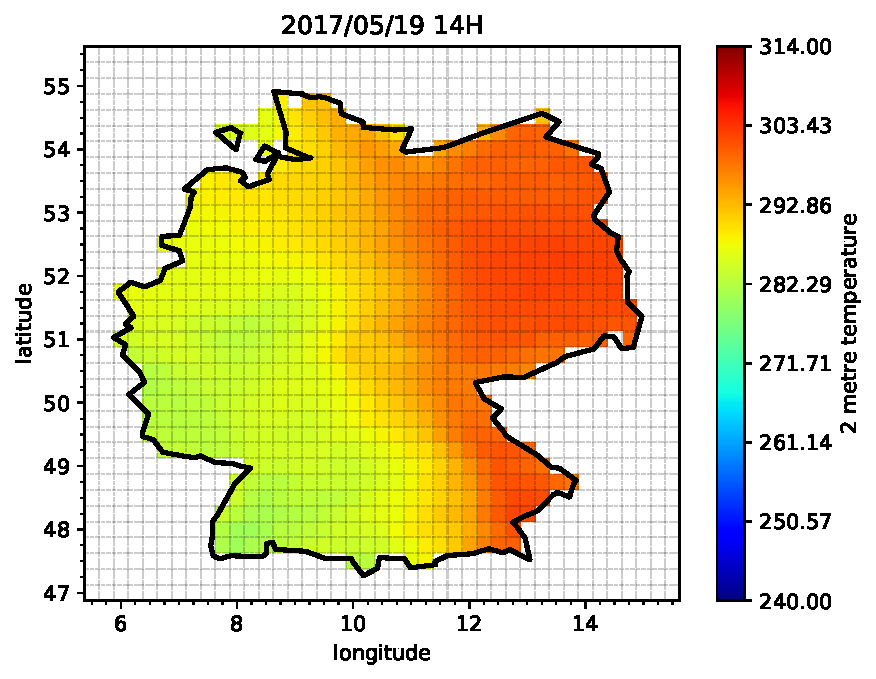
\includegraphics[width=.95\textwidth]{../doc/plots/t2m/maxvar/0_map_isin}%
		\label{fig:t2m_maxvar_0_map_isin}%
	\end{subfigure}
	\label{fig:isin_compare}
\end{figure}

\end{frame}


\begin{frame}{Evaluation II}

Stuffy stuff.

\begin{figure}[h!]%
\centering
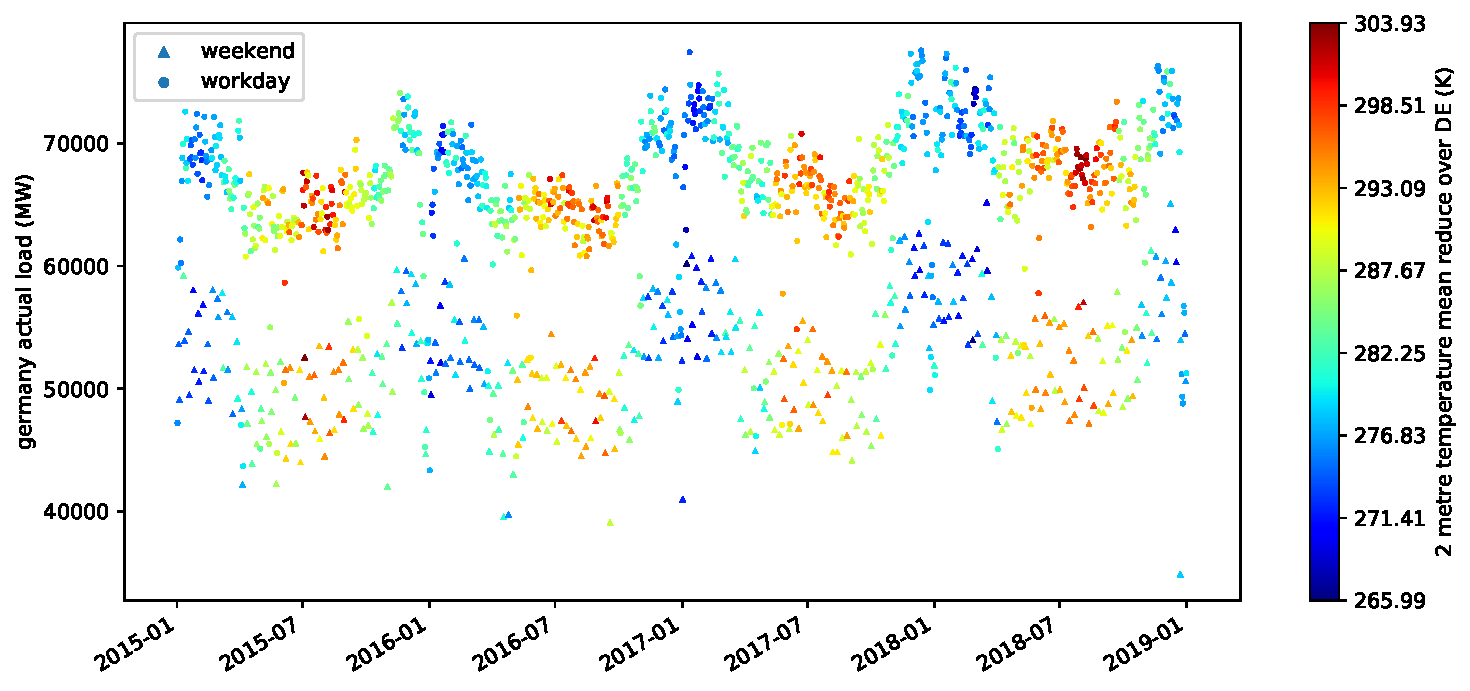
\includegraphics[width=\textwidth,origin=c]{../doc/plots/t2m_mean_2015010112_2018123112_24F}%
\end{figure}

\end{frame}


\begin{frame}{Evaluation III}

Wing stuffy\footnote{\url{https://wingware.com/}}. optional, max 30s%Be no wowy, mesa no talk much about disa.

\begin{figure}[h!]%
\centering
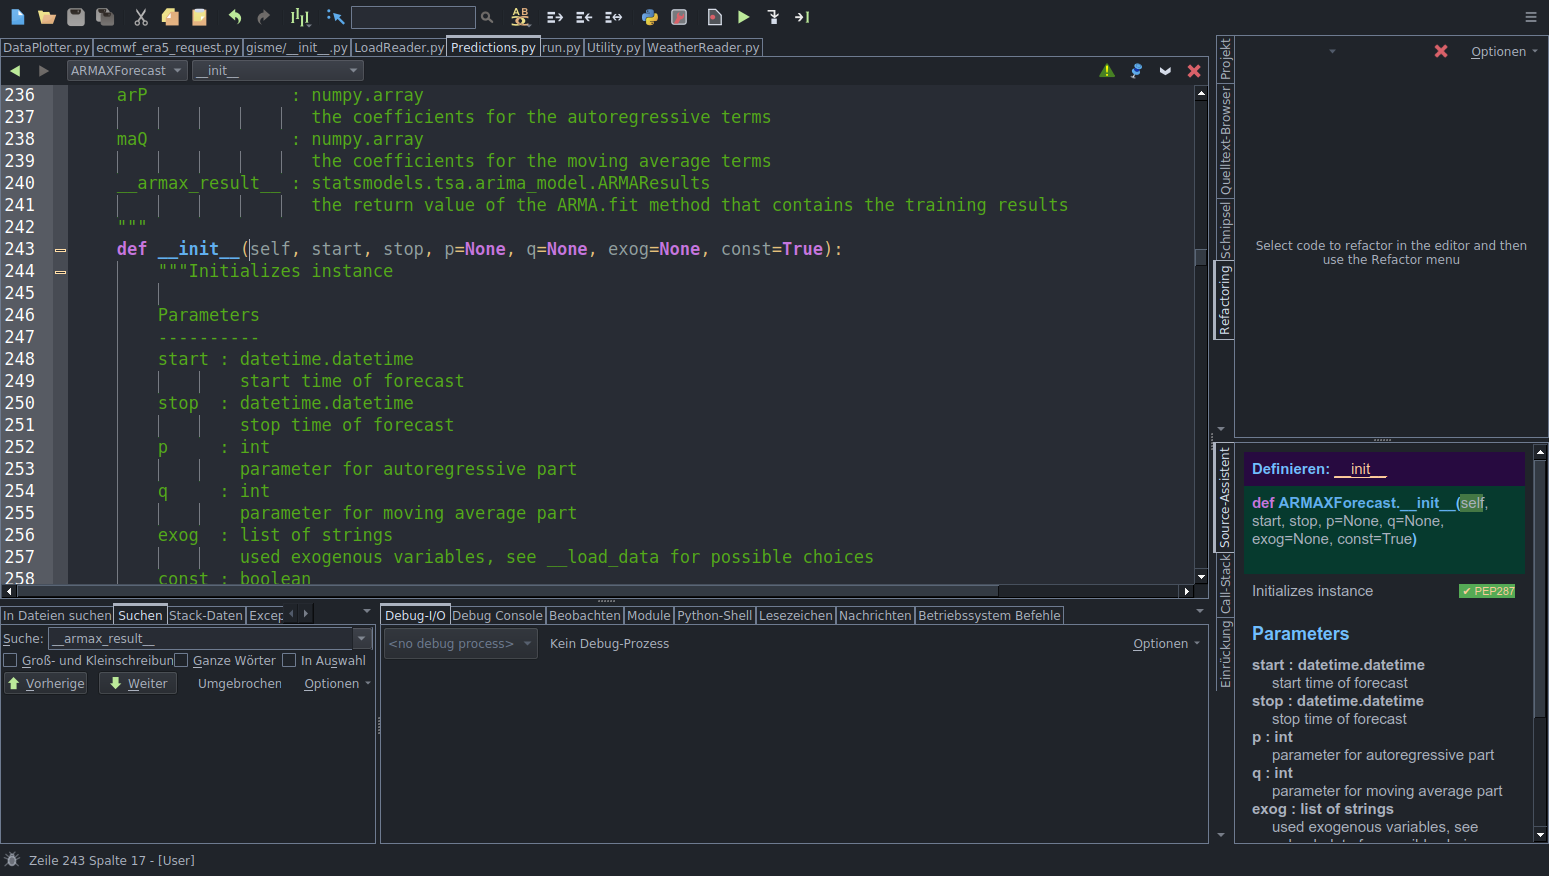
\includegraphics[width=.8\textwidth]{../doc/logos/Predictions_Wing_001}%
\end{figure}

\end{frame}


\begin{frame}{Evaluation IV}

Autocorrelation and partial autocorrelation function.

\begin{figure}[h!]%
	\centering
	\begin{subfigure}{.5\textwidth}
		\centering
		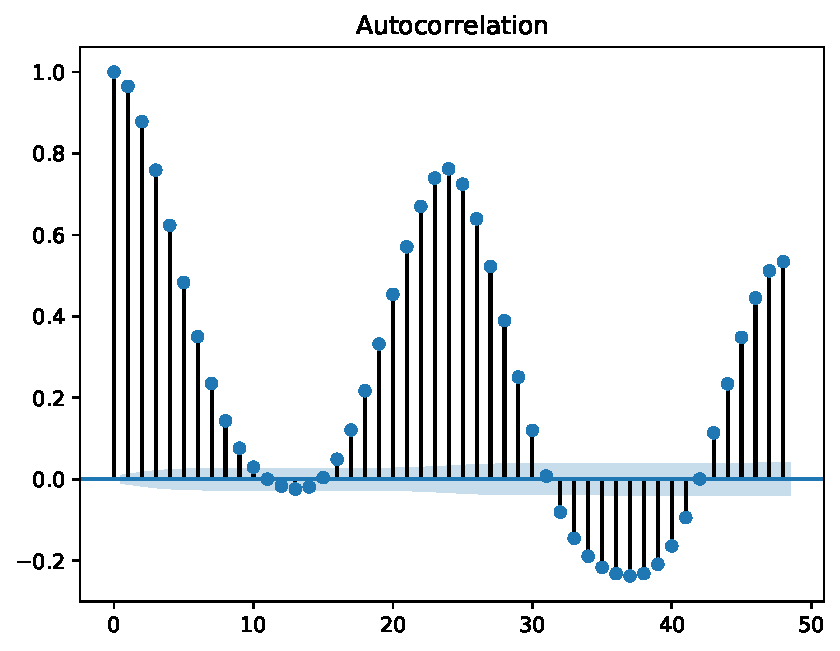
\includegraphics[width=\textwidth]{../doc/plots/ACF/load_48lags_ndiff0_hstep1}%
		\label{fig:acf_load_lags48}%
	\end{subfigure}%
	\begin{subfigure}{.5\textwidth}
		\centering
		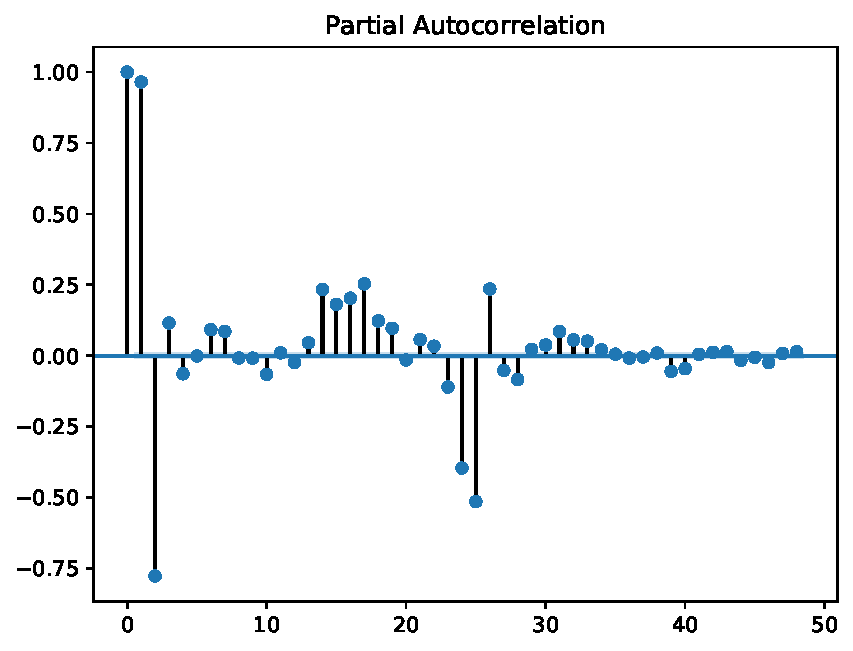
\includegraphics[width=\textwidth]{../doc/plots/PACF/load_48lags_ndiff0_hstep1}%
		\label{fig:pacf_load_lags48}%
	\end{subfigure}
\end{figure}

\end{frame}


\begin{frame}{Evaluation V}

\begin{table}
\rowcolors{2}{white}{gray!25}
\centering
\footnotesize
\begin{tabularx}{\linewidth}{p{.6cm}p{.6cm}XXXXXX}
& \textbf{MA(q) >\newline AR(p) v} & 0 & 1 & 2 & 3 & 4 & 5\\\hline
AIC\newline ~BIC\newline \rule{0pt}{1em}HQIC & 1 & 489489.23\newline 489513.76\newline 489497.15 & 472851.05\newline 472883.76\newline 472861.61 & 467543.07\newline 467583.96\newline 467556.27 & 466091.08\newline 466140.14\newline 466106.92 & 465622.11\newline 465679.35\newline 465640.59 & 464728.34\newline 464793.76\newline 464749.47\\
AIC\newline ~BIC\newline \rule{0pt}{1em}HQIC & 2 & 464699.50\newline 464732.21\newline 464710.06 & 464253.96\newline 464294.85\newline 464267.16 & 464204.94\newline 464254.01\newline 464220.79 & 464190.14\newline 464247.39\newline 464208.63 & 464054.46\newline 464119.87\newline 464075.58 & 463634.12\newline 463707.72\newline 463657.89\\
AIC\newline ~BIC\newline \rule{0pt}{1em}HQIC & 3 & 464324.69\newline 464365.58\newline 464337.89 & 464226.02\newline 464275.09\newline 464241.87 & 464202.92\newline 464260.16\newline 464221.4 & 463643.15\newline 463708.57\newline 463664.27 & 462483.99\newline 462557.59\newline 462507.75 & 462271.48\newline 462353.25\newline 462297.88\\
AIC\newline ~BIC\newline \rule{0pt}{1em}HQIC & 4 & 464171.28\newline 464220.35\newline 464187.13 & 464173.25\newline 464230.49\newline 464191.73 & 462433.17\newline 462498.59\newline 462454.29 & 462985.37\newline 463058.97\newline 463009.14 & 462149.01\newline 462230.78\newline 462175.41 & -\\
AIC\newline ~BIC\newline \rule{0pt}{1em}HQIC & 5 & 464173.18\newline 464230.42\newline 464191.66 & 463588.38\newline 463653.80\newline 463609.50 & 462944.78\newline 463018.38\newline 462968.54 & - & 462138.70\newline 462228.65\newline 462167.74 & -\\
\end{tabularx}
\label{tab:ic_table}
\end{table}

\end{frame}


\begin{frame}{Evaluation VI}

%Only load ARMA(2,2) from 2017/12/31 to 2018/01/08 using load data from 2015/01/080 to 2017/12/31 for training.

\begin{figure}[h!]%
\centering
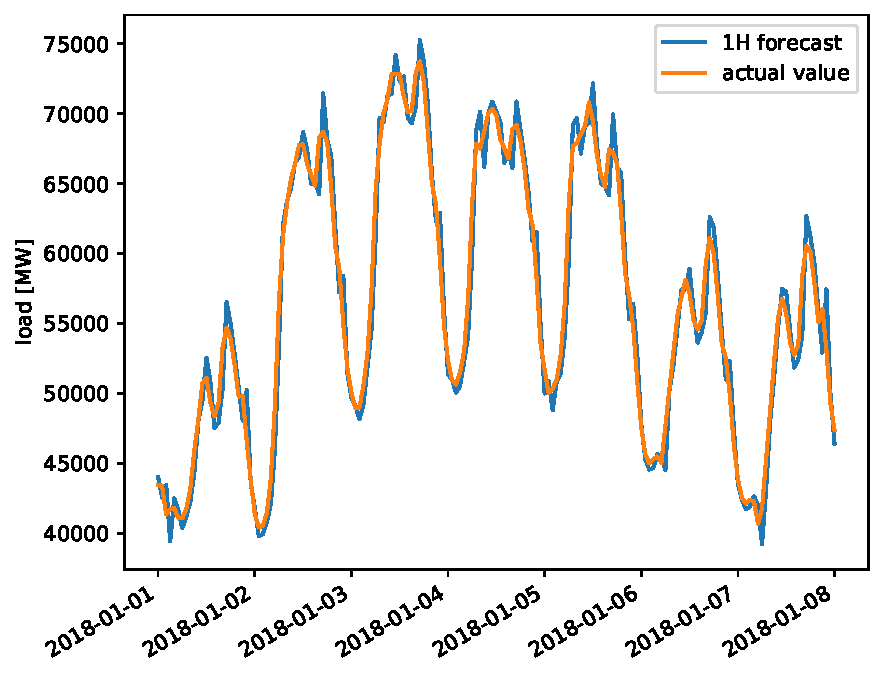
\includegraphics[height=\textheight]{../doc/plots/ARMAXfc/ARMAX_p2q2_data2015to2017_fcto2018123100_plot_range2018010100_2018010800}%
\end{figure}

\end{frame}


\begin{frame}{Evaluation VII}

%Forecast from 2017/12/31 to 2018/01/08 for ARMAX(2,2) with load data from 2015/01/08 to 2017/12/31 for train and grid points of ten regions with highest pop as exog.

\begin{figure}[h!]%
\centering
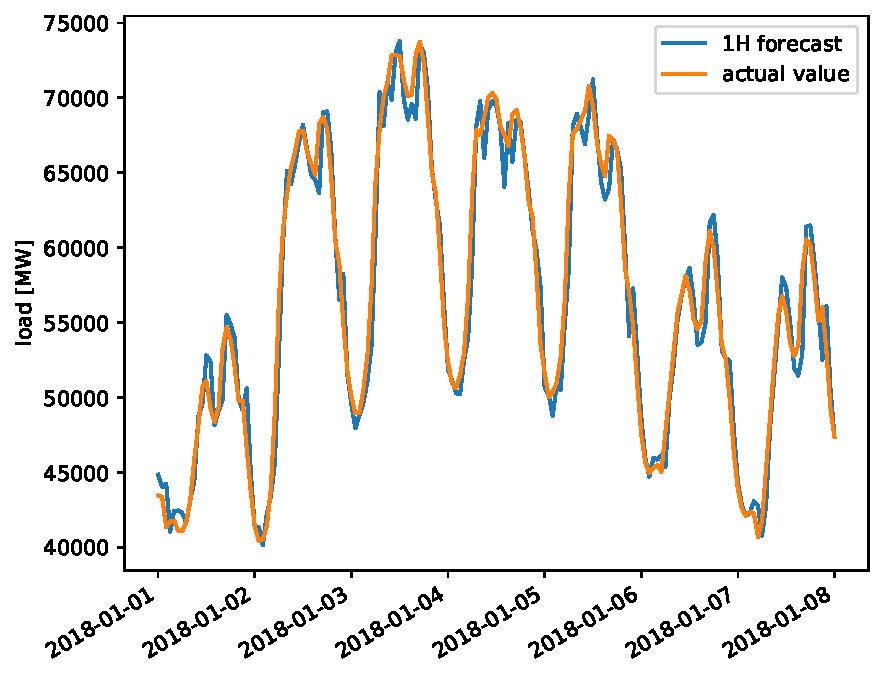
\includegraphics[height=\textheight]{../doc/plots/ARMAXfc/ARMAX_p2q2_data2015to2017_fcto2018123100_t2m_top10_plot_range2018010100_2018010800}%
\end{figure}

\end{frame}


\begin{frame}{Evaluation VIII}

%forecast from 2017/12/31 to 2018/01/08 for ARMAX(2,2) with load data from 2015/01/08 to 2017/12/31 for train and load data shifted back in time by 1 week for same time range as exog.

\begin{figure}[h!]%
\centering
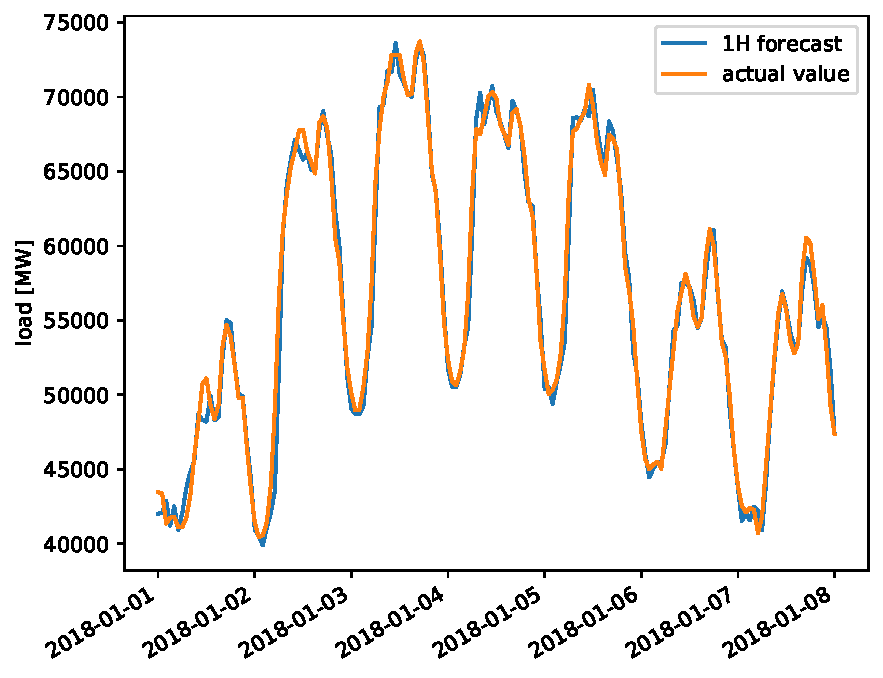
\includegraphics[height=\textheight]{../doc/plots/ARMAXfc/ARMAX_p2q2_data2015to2017_fcto2018123100_load_lag_plot_range2018010100_2018010800}%
\end{figure}%

\end{frame}


\begin{frame}{Evaluation IX}

%Forecast from 2017/12/31 to 2018/01/08 for ARMAX(1,0) with load data from 2017/01/01 to 2017/12/31 for train and all 1435 grid points of the t2m variable as exog.

\begin{figure}[h!]%
\centering
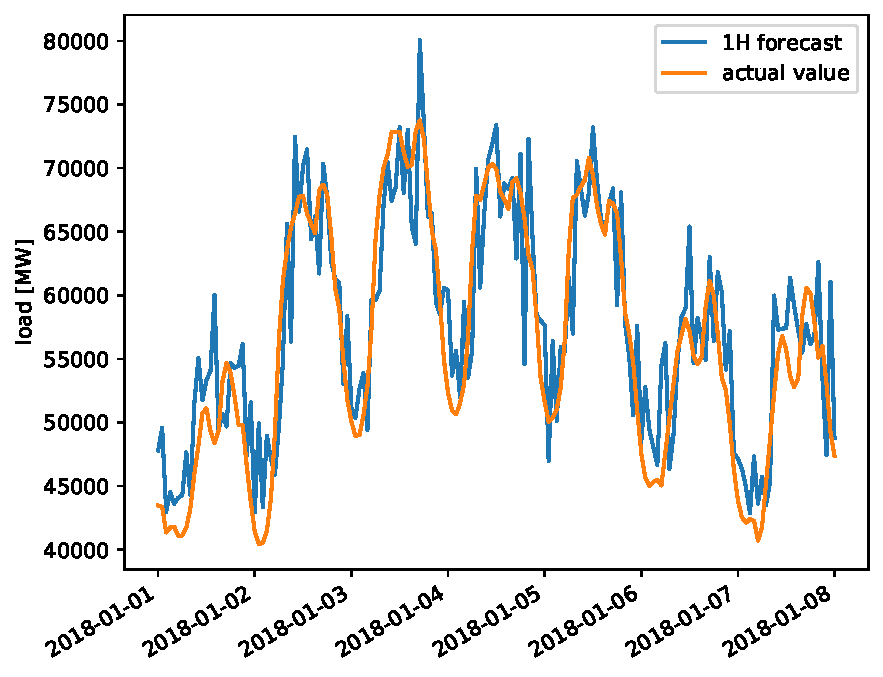
\includegraphics[height=\textheight]{../doc/plots/ARMAXfc/ARMAX_p1q0_data2017010100to2017123100_fc2017123101to2018010800_t2m_all}%
\end{figure}%

\end{frame}


\begin{frame}{Evaluation X}

\begin{table}[!ht]%
\rowcolors{2}{white}{gray!25}
\centering
\scriptsize
\begin{tabularx}{\linewidth}{Xlllllrrrr}
\textbf{model} & \textbf{1} & \textbf{2} & \textbf{3} & \textbf{4} & \textbf{5} & \textbf{RMSE} & \textbf{MAE} & \textbf{MPE} & \textbf{MAPE}\\\hline
ARMA(1,0) & \xmark & \xmark & \xmark & \xmark & \xmark & 2621.940 & 1961.213 & 0.006 & 3.460\\
ARMA(2,2) & \xmark & \xmark & \xmark & \xmark & \xmark & 1727.742 & 1216.559 & 0.220 & 2.114\\
ARMAX(2,2) & \cmark & \cmark & \xmark & \xmark & \xmark & 1024.265 & 628.298 & -0.020 & \cellcolor{green!35}1.103\\
ARMAX(2,2) & \cmark & \cmark & \cmark & \xmark & \xmark & 1024.310 & 628.331 & -0.006 & \cellcolor{green!35}1.103\\
ARMAX(2,2) & \cmark & \cmark & \xmark & \cmark & \xmark & \cellcolor{green!35}1024.251 & \cellcolor{green!35}628.292 & -0.020 & \cellcolor{green!35}1.103\\
ARMAX(2,2) & \cmark & \cmark & \cmark & \cmark & \xmark & 1024.295 & 628.324 & -0.006 & \cellcolor{green!35}1.103\\
ARMAX(2,2) & \cmark & \xmark & \xmark & \xmark & \xmark & 1030.753 & 633.436 & 0.101 & 1.112\\
ARMAX(2,2) & \cmark & \xmark & \xmark & \cmark & \xmark & 1030.756 & 633.433 & 0.101 & 1.112\\
ARMAX(2,2) & \cmark & \xmark & \cmark & \xmark & \xmark & 1029.191 & 633.093 & -0.165 & 1.114\\
ARMAX(2,2) & \cmark & \xmark & \xmark & \xmark & \cmark & 1043.292 & 649.564 & -0.018 & 1.144\\
ARMAX(2,2) & \cmark & \xmark & \cmark & \xmark & \cmark & 1043.711 & 650.046 & -0.012 & 1.145\\
ARMAX(2,2) & \cmark & \cmark & \xmark & \cmark & \cmark & 1051.801 & 659.805 & -0.021 & 1.165\\
ARMAX(2,2) & \cmark & \cmark & \cmark & \cmark & \cmark & 1051.956 & 660.006 & \cellcolor{green!35}-0.004 & 1.165\\
ARMAX(2,2) & \cmark & \xmark & \cmark & \xmark & \xmark & 1656.760 & 1178.435 & 0.021 & 2.043\\
ARMAX(2,2) & \xmark & \cmark & \xmark & \xmark & \xmark & 1662.298 & 1179.187 & 0.185 & 2.039\\
ARMAX(2,2) & \xmark & \cmark & \xmark & \cmark & \xmark & 1661.909 & 1179.681 & 0.187 & 2.040\\
ARMAX(2,2) & \xmark & \cmark & \cmark & \cmark & \xmark & 1656.224 & 1179.021 & 0.022 & 2.044\\
ARMAX(2,2) & \xmark & \cmark & \cmark & \cmark & \cmark & 1811.407 & 1321.255 & 0.043 & 2.315\\
ARMAX(2,2) & \xmark & \xmark & \cmark & \xmark & \cmark & 2004.932 & 1444.396 & -0.036 & 2.547\\
ARMAX(2,2) & \xmark & \xmark & \xmark & \xmark & \cmark & 2130.514 & 1508.978 & 0.211 & 2.663\\
%ARMAX(2,2) & \xmark & \xmark & \xmark & \xmark & \xmark & & & & \\
\end{tabularx}
\end{table}

1=shifted load,2=t2m mean,3=counter,4=weekend,5=top 10 regions t2m

\end{frame}


\againframe<5>{toc}


\begin{frame}{Conclusion}

Maybe use NN, RNN? At least, mention, that redundant information of grid-based data must somehow be filtered in order to improve forecasts and speed up computation.\\
\vspace{5mm}

\end{frame}

\begin{frame}{Summary}

Summ Summ Summ Summ Summ Summ Summ Summ Summ Summ\\
Lorem Summum.

\end{frame}

\begin{frame}
\vspace{26mm}\hspace{20mm}
{\Huge Acknowledgements}\\
\end{frame}


\begin{frame}[allowframebreaks]{References}
\printbibliography[heading=none]
\end{frame}


\end{document}
